\section{Aim 2. Elucidate the characteristics that determine sensitivity to oncogenic \KRAS{} mutations.}

\subsection*{Rationale}

Though \KRAS{} is estimated to be mutated in 10\%-14\% \cite{Bailey2018, Prior2020TheCancer} of all cancer, only a few cancer types frequently have oncogenic \KRAS{} mutations.
One explanation for this phenomenon is that the actual mutational event is less likely to occur in some tissues compared to others due to differences in mutagenic processes.
However, this is unlikely because neighboring tissues often demonstrate drastically different rates of \KRAS{} mutation.
One striking example is how 32\% of lung adenocarcinoma, but only 4\% of small cell lung cancer tumors have a \KRAS{} mutation \cite{Bailey2018, Prior2020TheCancer}.
Additionally, experimental evidence has demonstrated that even the forced expression of mutant \kras{} does not induce a hyperproliferative phenotype in all tissues \cite{Guerra2003TumorContext., Ray2011EpithelialModel,  Parikh2012MouseResponses}.
Instead, we hypothesize that the basal state of a tissue, including the existing signaling architecture, determines its sensitivity to \KRAS{} hyperactivation.
Therefore, we aim to identify properties of tissues that determine their sensitivity to \KRAS{}-driven oncogenesis.

%%%%%%%%%%%%%%%%%%%%%%%%%%%%%%%%%%%%%%%%%%%
% Aim 2.1
%%%%%%%%%%%%%%%%%%%%%%%%%%%%%%%%%%%%%%%%%%%

\subsection*{Aim 2.1. Determine the extent to which mutational processes affect the frequency of \KRAS{} mutations across multiple cancer types.}

\subsubsection*{Approach}

As mentioned previously, one explanation for the vast variation in \KRAS{} mutational frequency amongst different cancer types is that the causative mutations are more common in some tissues than others.

Mutational signatures will be used to assess the ability of various cancer types to obtain an oncogenic \KRAS{} mutation.
This will be accomplished via similar means as explained in Aim 1.1: by calculating the expected frequency of \KRAS{} mutations according to the genome-wide frequency of mutations in identical trinucleotide contexts.
However, instead of normalizing the values to report the probability of each allele to occur in each tumor sample, the values will be normalized to the total number of mutations in the tumor sample.
Thus, they will be comparable across cancer samples as a measure of the ability to gain a \KRAS{} mutation.

In addition, we will explore the use of count-based statistical models to extract additional information not available in aggregated statistics.
To begin, a logistic model will be fit to the number of mutations that could cause an activating \KRAS{} mutation and the total number of mutations to predict whether the tumor sample had a \KRAS{} mutation.
The coefficients of the fit model will be estimates of the impact of the types of mutations found in each sample on the probability of having a \KRAS{} mutation.
Additional models will be fit with fewer (e.g. just the total number of mutations) or additional (e.g. the mutation of other oncogenes such as \emph{BRAF} or \emph{EGFR}, stage of cancer, etc.) covariates to estimate the predictive power of the number of mutations that could create an oncogenic \KRAS{} allele taking into account other factors.
Additional models that include random effects for the tissue of origin or use a mixture-distribution to model different underlying rates of mutation can be compared to the logistic models.

Because there is experimental evidence that the tissue-of-origin determines the effect of hyperactive \kras{}, I expect that the number of mutations that could cause a \KRAS{} mutation will have little predictive power on whether a tumor sample has a \KRAS{} mutation.
Still, this analysis presents a rigorous statistical examination of this potential explanation.

\subsubsection*{Pitfalls and alternative approaches}

The proposed methods are limited in similar ways as mentioned in Aim 1.1.
Namely, this analysis will continue to assume that mutational forces act uniformly across the genome.
We can investigate the feasibility of using local rates and patterns of mutation to enhance the model as is done in many oncogene-predicting algorithms including \cite{  Lawrence2013, Tamborero2013, Dietlein2020IdentificationContext.}

An additional limiting factor of the analysis will be the sparsity of \KRAS{} mutants in tumors from \KRAS{}-insensitive tissues.
This will limit the number of cancer types that can be studied as only those with a sufficient number of \KRAS{} mutants can be fit with the logistic models.

\subsubsection*{Preliminary data}

Currently, I have collected the sequencing data of about 42,000 tumor samples from 32 different tissues of origin.
Of this data set, 13,652 samples have targeted sequencing data and the remaining 28,321 samples were either whole genome or exome sequenced (WG/ES).
These cancers have been anatomically organized using the OncoTree graph from Memorial Sloan Kettering (Figure \ref{fig:oncotree}).

\begin{figure}[t!]
\centering
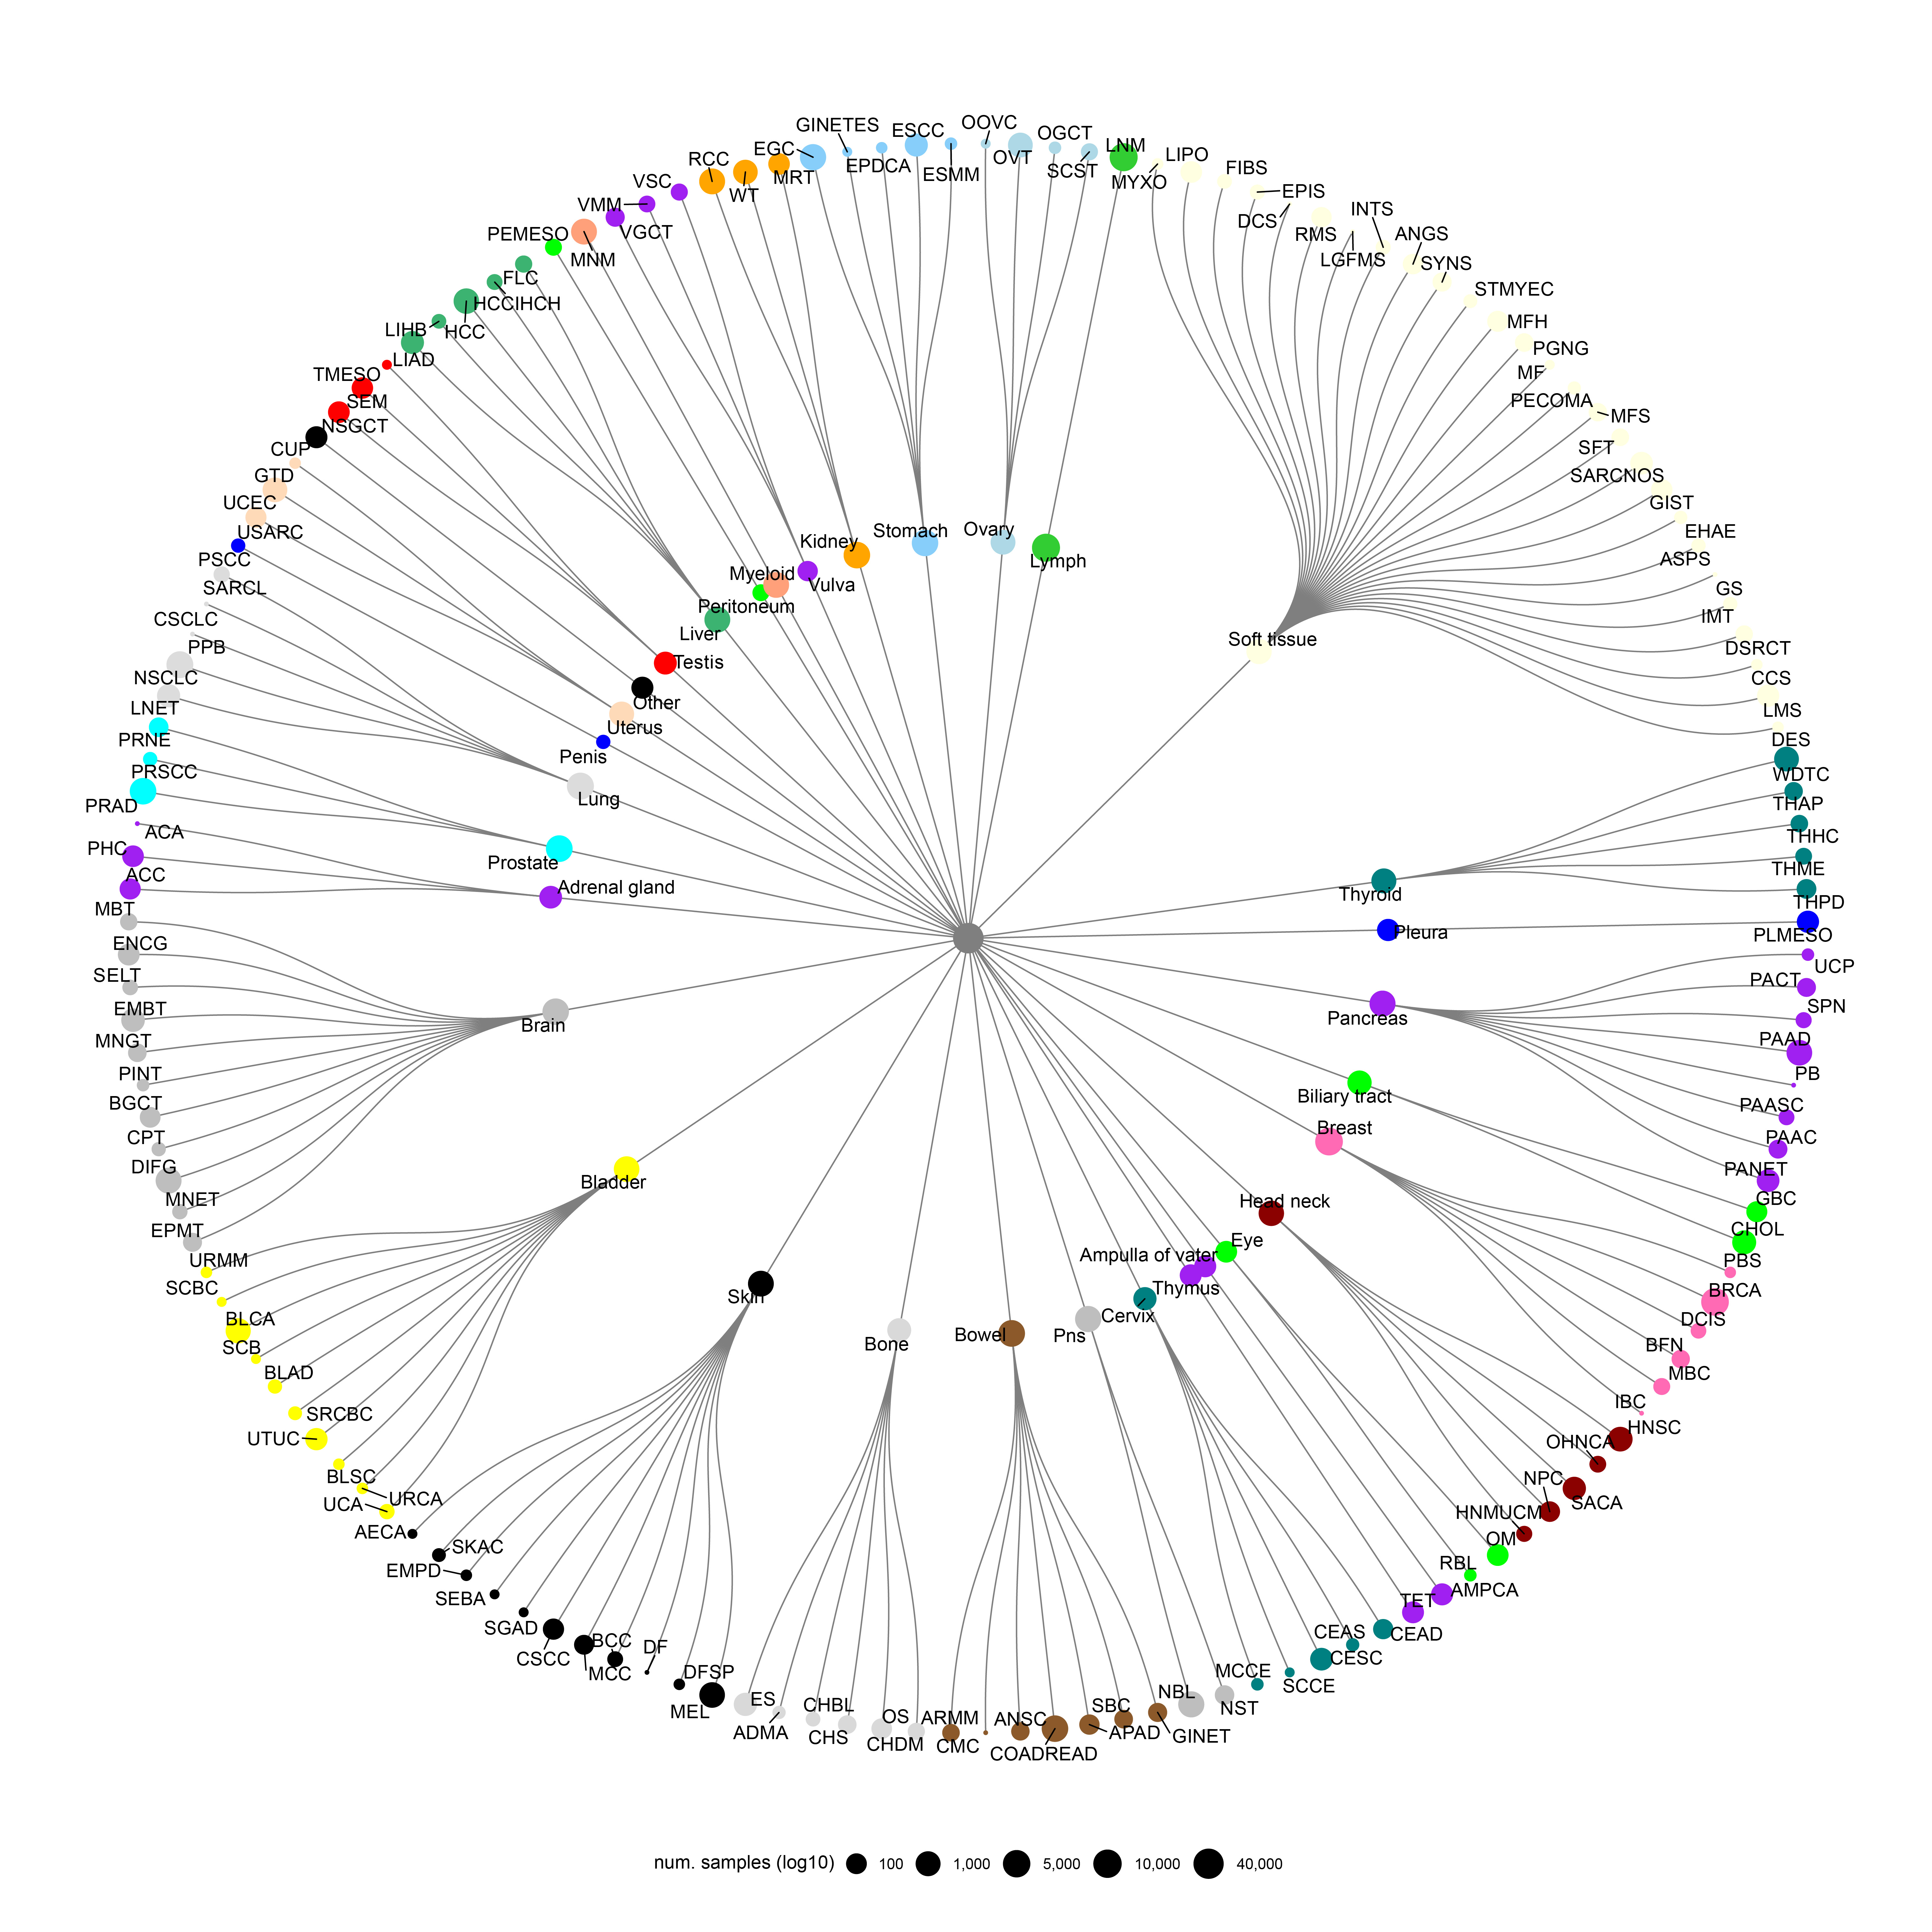
\includegraphics[width=180mm]{figures/aim2/oncotree_figure.jpg}
\caption{
    \textbf{The cancer samples were organized according to their anatomical relationships using the OncoTree.}
    Each layer from the middle represents a sub-location of the parent node.
    Nodes are colored by the parent organ and the size is related to the number of cancer samples that have been collected.
}
\label{fig:oncotree}
\end{figure}

As stated above, the number of \KRAS{} mutations will be a major determinant for whether mutation information from a cancer type can be analyzed as described.
Thus far, the \KRAS{}-insensitive tissues with the most number of samples with WG/ES data and an oncogenic \KRAS{} mutation include hepatocellular carcinoma, bladder urothelial carcinoma, cholangiocarcinoma, and esophagogastric adenocarcinoma (Figure \ref{fig:num-samples-kras-resistant}).

\begin{figure}[t!]
\centering
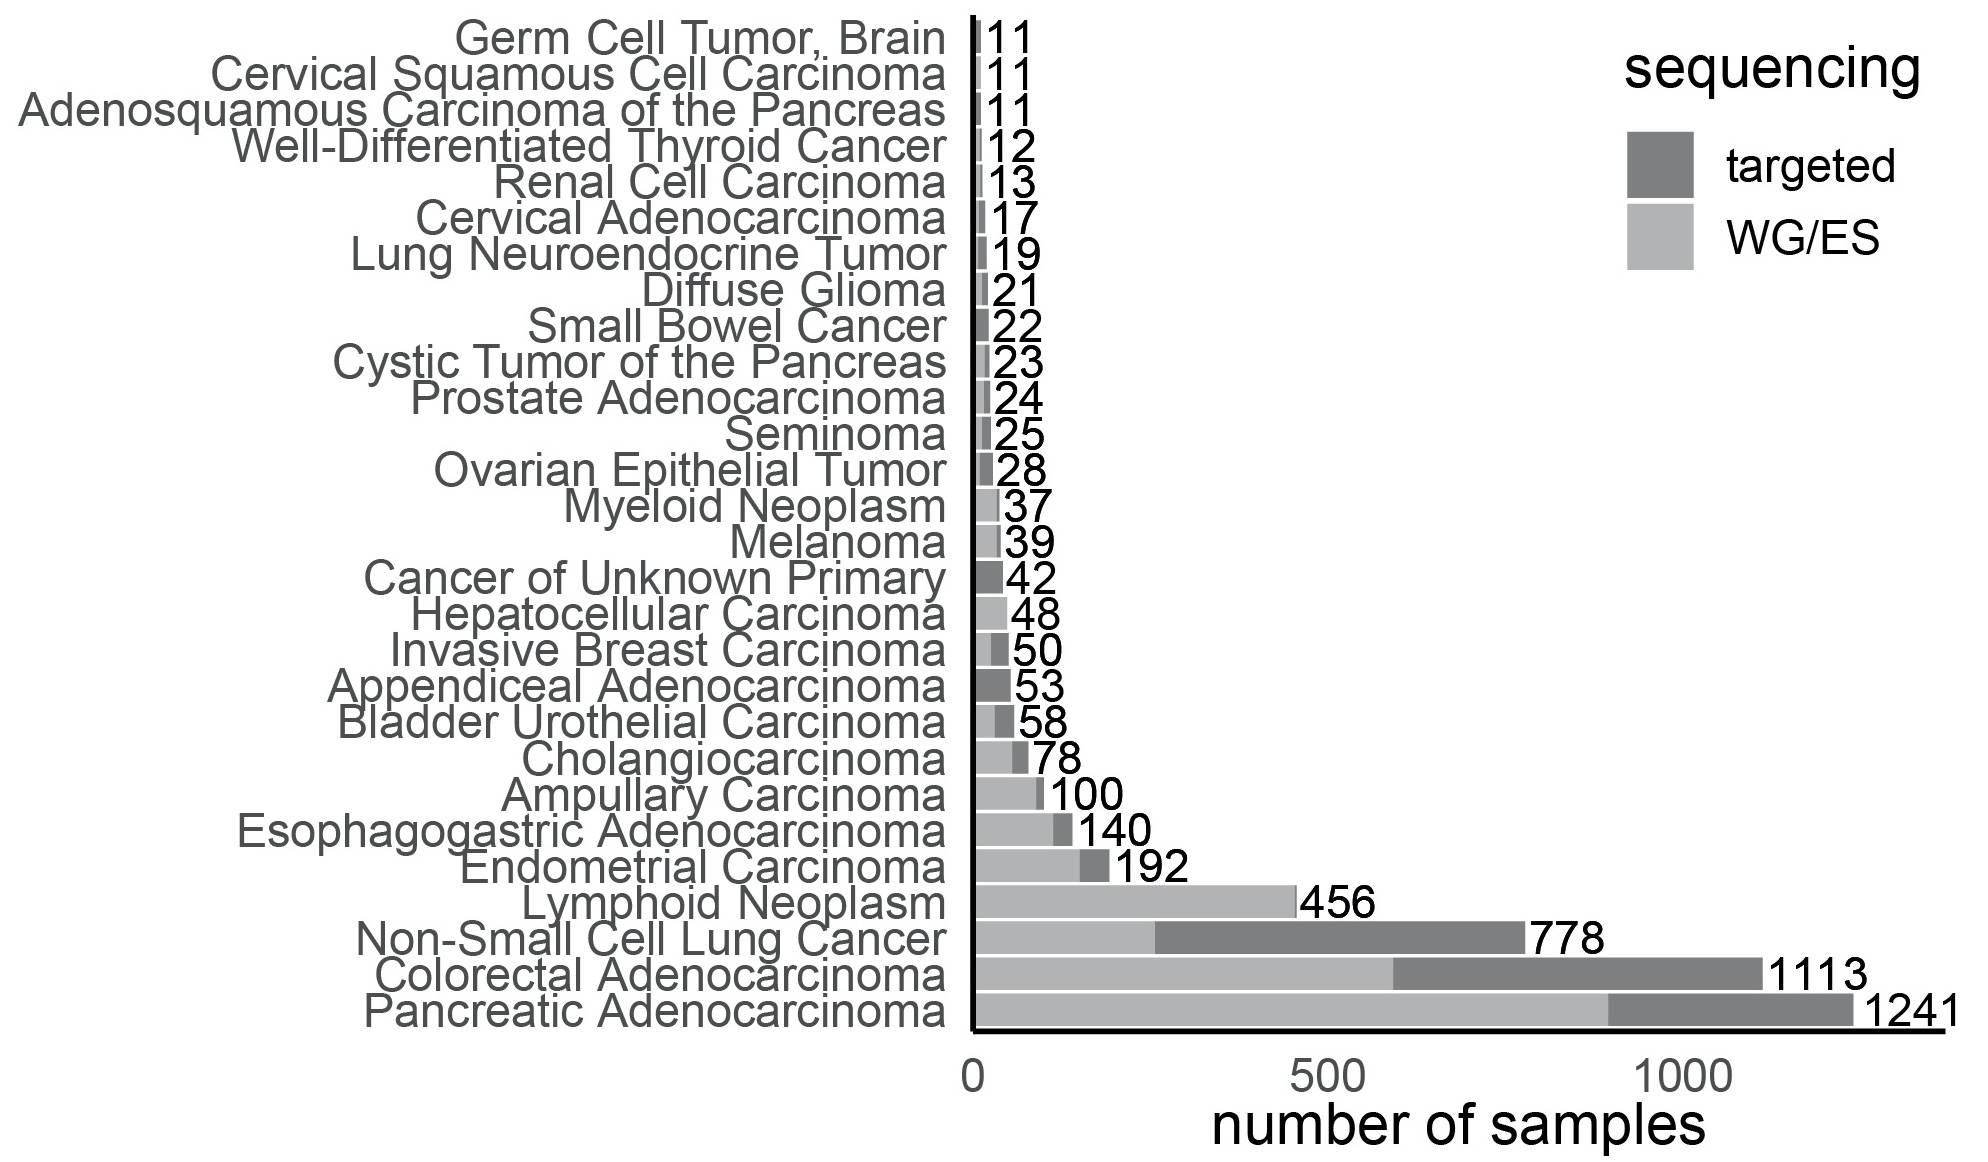
\includegraphics[width=120mm]{figures/aim2/kras-mutations-from-insensitive-tissues.jpg}
\caption{
    \textbf{The number of targeted sequenced and WG/ES samples with \KRAS{} mutations.}
    Each cancer type (row) is annotated with the total number of samples with a \KRAS{} mutation.
}
\label{fig:num-samples-kras-resistant}
\end{figure}

%%%%%%%%%%%%%%%%%%%%%%%%%%%%%%%%%%%%%%%%%%%
% Aim 2.2
%%%%%%%%%%%%%%%%%%%%%%%%%%%%%%%%%%%%%%%%%%%

\subsection*{Aim 2.2. Model \KRAS{} sensitivity on the basal signaling of a tissue.}

\subsubsection*{Approach}

Our hypothesis is that the structure of the ordinary signaling networks in a tissue determines its susceptibility to transformation by hyperactive \kras{} signaling.
Thus, I will use tandem-mass-tagged (TMT)-labeled \cite{Thompson2003} proteomic and phosphoproteomic data from \moKRAS{}\textsuperscript{WT/WT} mice collected by Dr. Olesja Popow to identify distinctions between sensitive and insensitive tissues.
The following organs were collected: colon, lung, pancreas, spleen (the "\KRAS{}-sensitive" tissues), heart, kidney, liver, skeletal muscle, and small intestine (the "\KRAS{}-insensitive" tissues).
The goal is to generate hypotheses that we could ultimately test in a mouse by pharmacologically or genetically modifying an insensitive tissue to make it sensitive to \KRAS{} mutation.

As before, I will model on whether or not the tissue is sensitive to \KRAS{} mutation. 
The amount of each protein, the amount of phosphorylation of each protein, the level of phosphorylation relative to the total amount of each protein, and ratios of different phosphorylations on the same protein can be used as input values.

Unless directly addressed, the high dimensionality of the data will cause the model to overfit.
As such, three strategies will be tested.
First, proteins that are involved in key signaling pathways (such as Wnt regulation, the MAPK pathway, or cell cycle regulation) will be manually selected.
Second, regularization or stepwise model selection algorithms will be used to reduce the number of predictors to just those with the most explanatory value by penalizing model complexity \cite{Tibshirani1996RegressionLasso., Zou2005RegularizationNet}.
Third, latent-variable models such as partial least squares, principal component regression, or factor analysis will be tested.
These groups of methods provide a comprehensive comparative analysis of the many potentially explanatory models for the data.

\subsubsection*{Pitfalls and alternative approaches}

One limiting factor of the analysis will be the relatively few data points collected.
Twelve mice total were sacrificed, but, to increase the amount of protein for detection by mass spectrometry (MS) and reduce variation between samples, four mice (two females and two males) were pooled for each 10-plex set of TMT-labeling.
Therefore, there are only 3 data points per protein per tissue.

The approach outlined above uses only linear models, though there are many non-linear models that could be used to identify differences between the two groups of tissues, such as support vector machines and random forest classifiers.
There are two primary reasons why we propose the use of linear models for the present study.
The first is that we believe that coefficients for the linear methods are more interpretable than the parameters used by non-linear methods.
The second is that the nonlinear methods have hyperparameters that must be tuned to prevent overfitting.
With so few data points, common methods, such as cross-validation, are not as effective.

A potential pitfall for this analysis is that \KRAS{} may not drive cancer via the same mechanism in all \KRAS{} sensitive tissues.
Conversely, the same may be true for how insensitive tissues stifle oncogenic \kras{} signaling.
Therefore, we will also build models using subsets of the tissues.
Subsets could include comparing a single sensitive tissue to all of the insensitive tissues, or comparing tissues of similar function but different sensitivity to \KRAS{} (such as the colon and the small intestine).

% These are mice and not humans. Tie in human information in the next sub-aim

\subsubsection*{Preliminary data}

As mentioned above, the proteomics and phosphoproteomics data have been collected for three groups of four mice.
Unsurprisingly, a preliminary exploratory analysis indicated that the strongest similarities are between samples of the same organ.
When the dimensionality of the protein-space was reduced by PCA, plotting the t-SNE of the new dimensions demonstrated that the samples from the same organ clustered together (Figure \ref{fig:proteomics-eda}a, b).
Additionally, using a Student's \emph{t-test} to find the proteins that most clearly distinguished between the sensitive and insensitive tissues instead identified proteins with high tissue-specific expression (Figure \ref{fig:proteomics-eda}c).
These two precursory analyses demonstrate that organ-specific expression will present a major difficulty in finding relevant distinctions between the proteomics of sensitive and insensitive tissues.

\begin{figure}[ht]
\centering
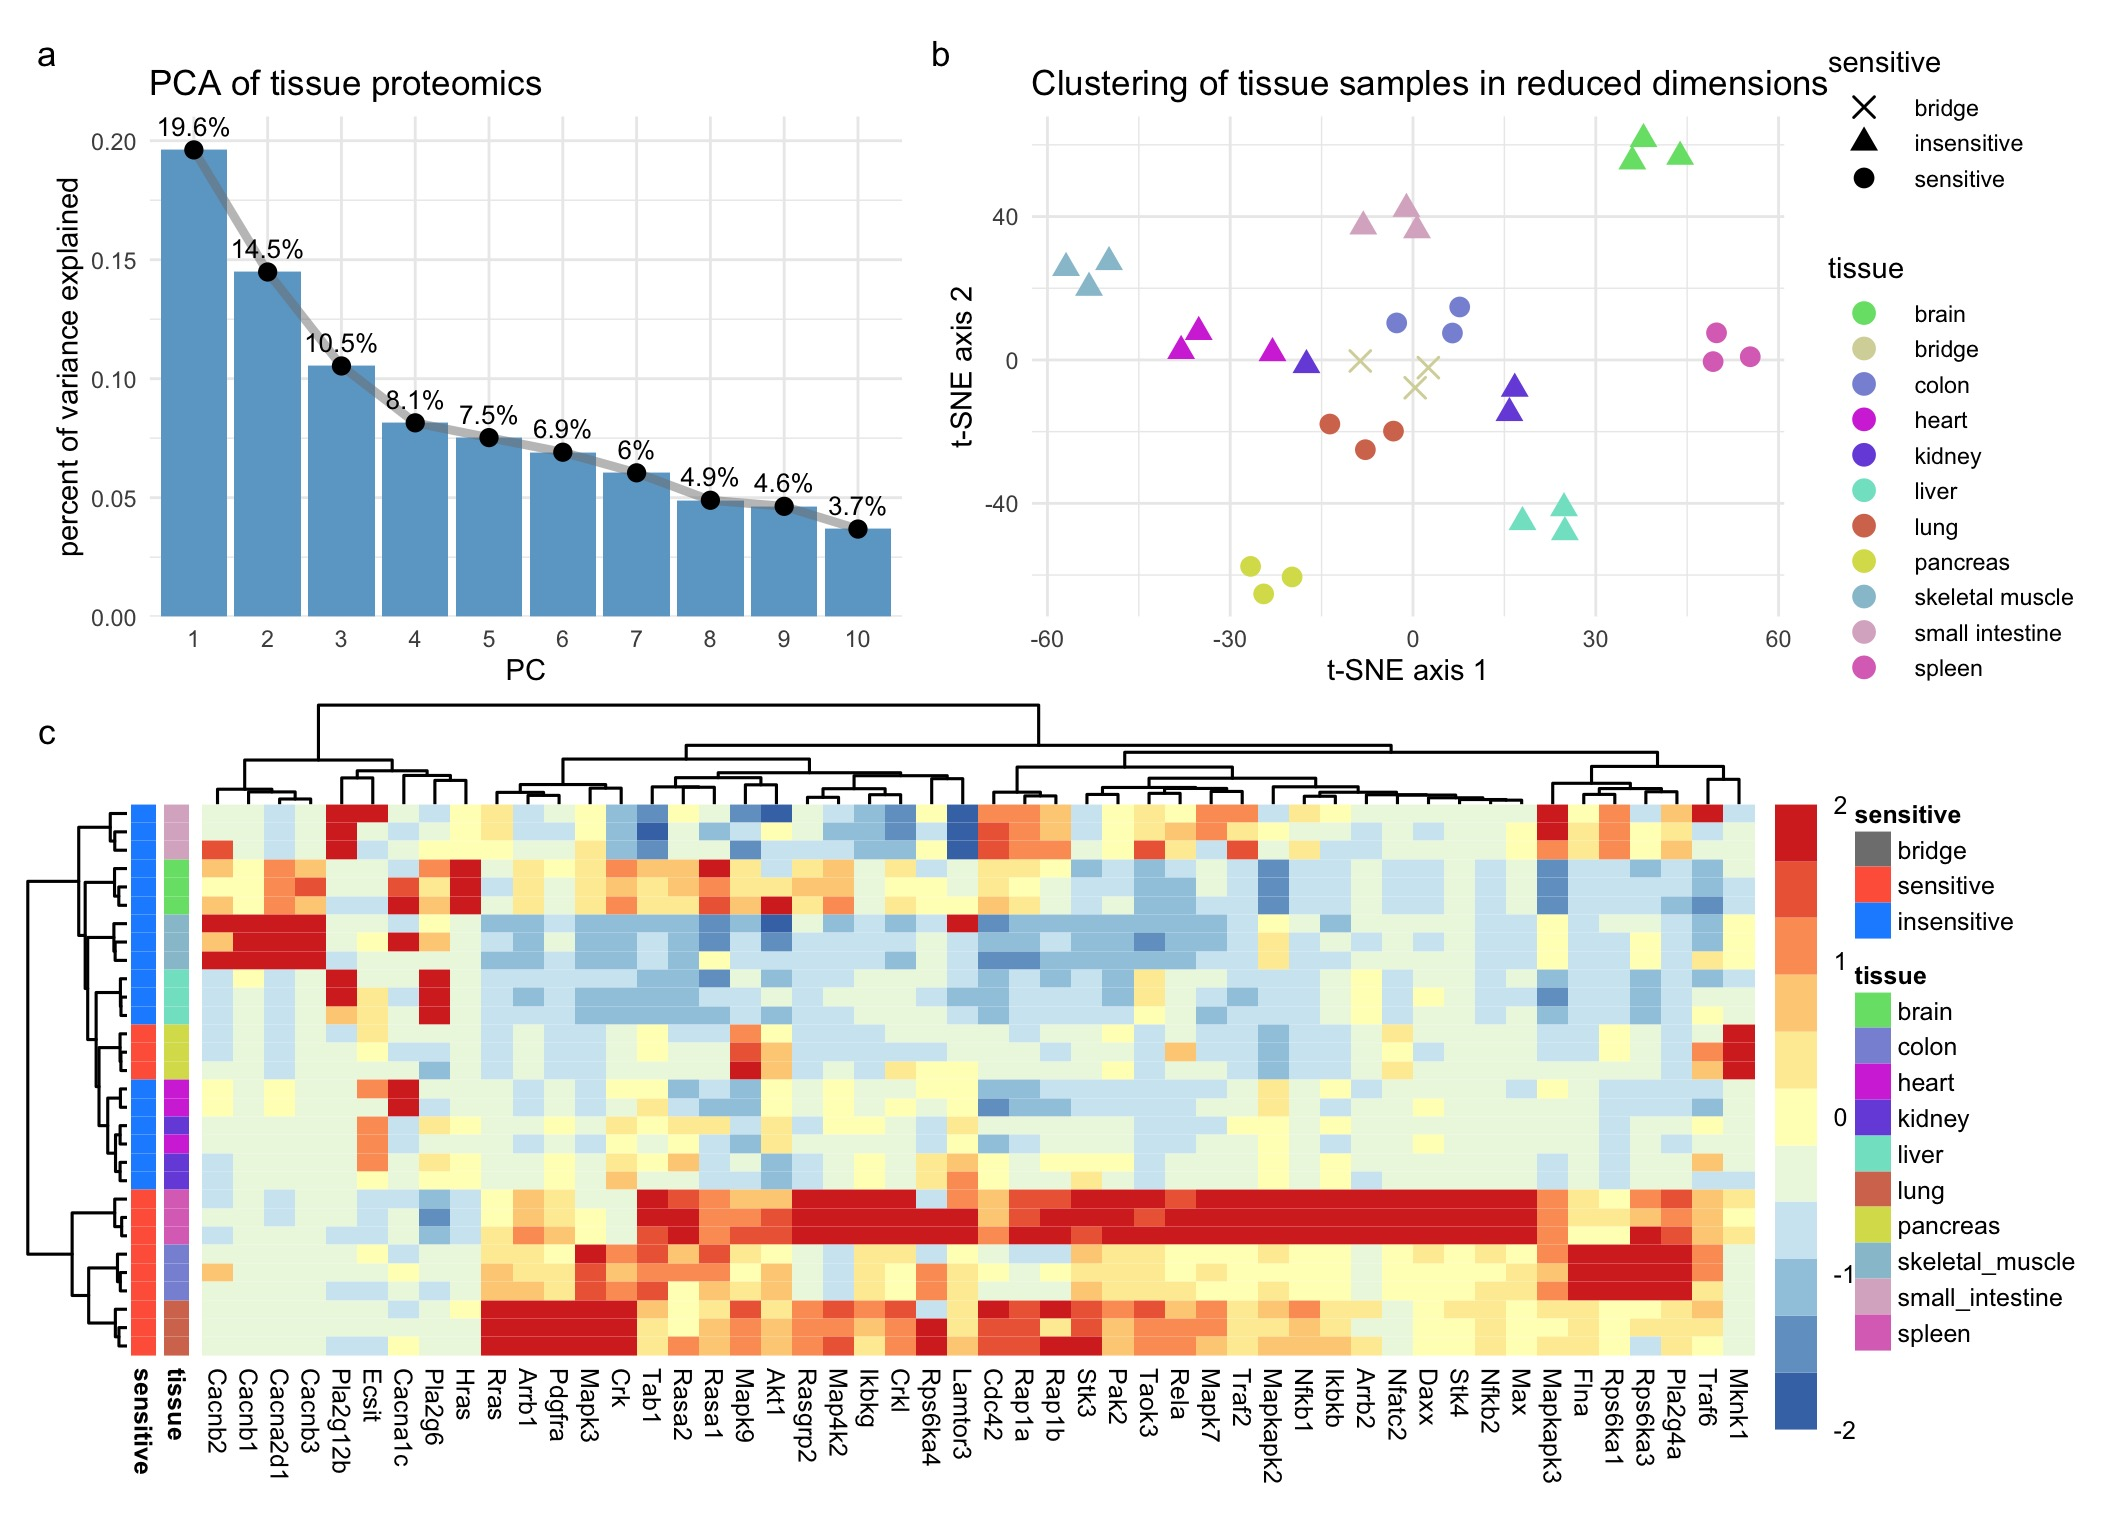
\includegraphics[width=180mm]{figures/aim2/proteomics-eda_figure.jpeg}
\caption{
    \textbf{The proteomics data cluster by tissue-type, not \KRAS{}-sensitivity.}
    \textbf{a.} The variance explained by the first ten principle components (PC) of the proteomics data.
    \textbf{b.} t-SNE applied to the new coordinates from PCA. Each point is colored according to the tissue and indicated to be \KRAS{}-sensitive or -insensitive by a circle or triangle, respectively. The bridge channels are indicated by "x"-marks.
    \textbf{c.} A heatmap of the 50 proteins with the strongest differences between sensitive and insensitive tissues (Student's \emph{t}-test, selected by p-value). Each column is a protein and each row is a tissue sample with the tissue and \KRAS{} sensitivity labeled by the column annotation.
}
\label{fig:proteomics-eda}
\end{figure}


%%%%%%%%%%%%%%%%%%%%%%%%%%%%%%%%%%%%%%%%%%%
% Aim 2.3
%%%%%%%%%%%%%%%%%%%%%%%%%%%%%%%%%%%%%%%%%%%

\subsection*{Aim 2.3. Identify recurring events in insensitive tissues with oncogenic \KRAS{} mutations.}

\subsubsection*{Approach}

Though the experimental evidence suggests that some tissues are not susceptible to hyperactive \kras{} signaling, there are still tumors from these locations that possess a mutation at a \KRAS{} hotspot.
While Aim 2.2 proposes to identify the differences between \KRAS{}-sensitive and insensitive tissues at homeostasis, this Aim approaches the question from the opposing direction: "What allowed \KRAS{} to drive these cancers in normally insensitive tissues?"

First, we will determine if these mutations were likely to have driven the cancer by measuring their allele-fraction in the sequencing data.
If the mutation to \KRAS{} was found in a small proportion of the sequencing reads that covered the \KRAS{} locus (compared to mutations of \emph{bona fide} oncogenes of the cancer), then it was less likely to have driven tumor progression and was instead a passenger mutation.
In addition, if the data are available, we can analyze RNA and/or protein expression to ensure that the hyperactive allele was expressed.

If we find that the \KRAS{} mutations were likely to have acted as drivers in tumors originating in insensitive tumors, the we will proceed with characterizing recurrent genetic co-alterations.
This would include a comutation analysis similar to that described in Aim 1.2 to identify genes that tend to comutate with \KRAS{}.
Also, because the loss of tumor suppressor genes is important to the progression of \KRAS{}-driven cancers (e.g. the loss of \emph{APC} in COAD, \emph{STK11} and \emph{KEAP1} in LUAD, and \emph{CDKN2A} in PAAD), we will analyze the co-occurrence of copy number alterations (CNA) to known tumor suppressors.

Finally, we will use the conclusions from this analysis of human data to help understand the models in Aim 2.2.
As the models are looking for differences between multiple organs, it will be difficult to tell what is distinct due to tissue-specific functions and what is relevant to \KRAS{} sensitivity.
Thus, knowing what permitted an insensitive tissue to be transformed by a \KRAS{} mutation in human tumors will help interpret the findings from Aim 2.2.

\subsubsection*{Pitfalls and alternative approaches}

As noted in Aim 2.1, the sparsity of \KRAS{}-mutants tumors from \KRAS{}-insensitive tissues will be a limiting factor.
It will introduce a limit on the power of the analysis to detect more rare comutation events.

\subsubsection*{Preliminary data}

So far, I am still collecting and preparing data for analyses.
An overview of the number of tumor samples and how many have \KRAS{} mutations were displayed in Aim 2.1.

% \subsection*{Vinay's notes on Aim 2}

% {\color{red}
% \begin{enumerate}
% \item Aim 2.1 is unclear in describing your approach to use mutational signatures for determining which mutational processes alter KRAS mutational frequency. Conceptually, it seems like you are relating the strength of mutational signatures in each sample to the frequency of KRAS alleles relative to the number of mutations per tumor sample. It's not clear how this would be different from Aim 1.1 and how this would provide something different from what you already found out in Figures 3.1 and 3.2. Although all of the relevant mutations in KRAS are nonsynonymous, I think you also need to account for the overall rates of synonymous and nonsynonymous mutations observed across the genome (you may have already done so) in both your mutational signature calculation and your logistic model. If tumor types exhibit variation int he balance between nonsynonymous mutations and fewer synonymous changes, then you will need to account for whether a mutational process that may generate KRAS mutants would tend to generate more synonymous than nonsynonymous mutations. I also think that mutational signature strengths and exposures would be relevant covariates for the logistic model. You should include a few sentences about how you intend to select covariates for your logistic model and how you will control for false associations.

% \item If tissue-of-origin is experimentally shown to be a major covariate, you could test for the associations of chromatin state upon KRAS severity in this Aim (unless you have already tested this). Polak et al Nature 2015 (https://www.nature.com/articles/nature14221) and more recently https://www.biorxiv.org/content/10.1101/517565v1 conduct tests about precancerous mutations occurring in the genome marked with tissue-specific chromatin modifications and find an associations between where those mutations occur and what type of tumor one gets. You propose taking a similar approach in Aim 3, but I think you should examine chromatin structure and correlation to the occurrence and ellele-frequency of a specific KRAS allele as well. You could also test if you could find an association between what KRAS allele your sample has in what tissue type and where the genome-wide mutations occur -- if tissue type should dictate which KRAS allele you get, then other features of tissue type should correlate with the KRAS allele as well. This test could fix the issue of loss of predictive power for your model. You could use Roadmap Epigenome chromatin annotations from matched normal tissue type or TCGA ATAC-seq for tumor-specific chromatin accessibility. 

% \item Are you going to use matched-normal data and/or normal mutation rates in tissue as a control for associations of a mutational signature to a nonsynonymous mutation? If you are making the claim of a particular mutational process in one tissue driving the formation of a specific KRAS allele or mutations to the other interacting components, you would need some control for 

% \item For the proteomics, you need to include a small piece about how you can benchmark the sensitivity of protein detection. MS/MS still has issues with detecting proteins at levels proportional to their concentration (in most MS/MS experiments, maybe a handful of peptides in a larger protein sequence get detected), and while normalization strategies exist, you should include in your "pitfalls" section for Aim 2.2 how you will account for dropped-out proteins and the loss of sensitivity to detect a protein involved in KRAS allele activity. For instance, will you construct a saturation curve to determine if downsampling PSMs at a certain fraction will cause some proteins to completely drop out of detection? Will you use transcriptomics to help support whether a protein is truly dropped out? Are you going to fit some kind of standardized value of protein abundance instead of actual abundance values?

% \item For 2.3, you will need to compare KRAS's allele frequencies to the frequencies estimated for driver point mutations -- I'd recommend reading the PCAWG papers on driver mutations (https://www.biorxiv.org/content/10.1101/190330v2, https://www.ncbi.nlm.nih.gov/pmc/articles/PMC7002750/) to get a sense of how exactly you could infer driver or passenger status from allele frequencies. To start, if you are working with the PCAWG data, then allele frequencies for known drivers and passengers of different somatic mutations will have already been determined, and you can use those results to construct a simple model for what passenger/neutral KRAS mutation allele frequencies will look like vs driver/functional KRAS mutations. You should also compare the results to those of mutations at other critical signaling proteins (EGFR, MAPK, etc). 

% \item Amiddst all of this, how are (if at all) controlling for copy number status?

% \item It is not clear from Aim 2.3 how much power you would have to find KRAS alleles in insensitive tissues because the overall model of KRAS sensitivity that you are suggesting implies that most of the functional KRAS alleles are largely found in sensitive tissues and not at significant levels in insensitive tissue (unless you actually have those measurements in other tumor types). If you can't detect KRAS mutations in insensitive tissue, how could DepMap data provide a reasonable proxy for the co-mutation analysis? I think we had discussed such an analysis last year, so I think it would be useful to include in your "pitfalls" section how you could use DepMap data (where KRAS "mutations" would have been experimentally induced in otherwise insensitive tissue). 

% \end{enumerate}
% }